% Presentación del video — Proyecto 3, Aprendizaje Maquinal (Saber 11 2025)
% Compilar: pdflatex presentacion.tex  (dos veces para los enlaces)
% Fuente de todos los números: informe/informe.pdf y results/2025/brechas.csv
\documentclass[aspectratio=169,11pt]{beamer}
\usepackage[utf8]{inputenc}
\usepackage[spanish]{babel}
\usepackage{graphicx}
\usepackage{booktabs}
\usetheme{Madrid}
\usecolortheme{default}
\setbeamertemplate{navigation symbols}{}
\setbeamertemplate{footline}[frame number]
\graphicspath{{../informe/fig/}}

\title{Hogar, colegio y municipio en Saber 11 de 2025}
\subtitle{Agrupación, árboles de decisión y bandits contextuales}
\author{Camilo Alejandro Lagos Malaver \and Luis Gabriel Peraza Muñoz}
\institute{Introducción a Sistemas Inteligentes, 2026-2 \\ Universidad Nacional de Colombia, Bogotá}
\date{9 de diciembre de 2026}

\begin{document}

\begin{frame}
  \titlepage
\end{frame}

\begin{frame}{El problema y los datos}
  \textbf{Preguntas:} ¿qué tipos de estudiantes y colegios existen? ¿qué predice
  quedar en la mitad superior? ¿puede un tutor virtual identificar el área más débil?
  ¿qué cambió frente a 2022?
  \vspace{0.4cm}
  \begin{itemize}
    \item Microdatos Saber 11 2025 (DataIcfes): 661.891 inscritos; 661.889 tras
    deduplicar; \textbf{561.049 estudiantes} de colegio con los cinco puntajes
    (21.675 del periodo 20251 y 539.374 del 20252).
    \item Cruce 1: IPM municipal del DANE 2018 --- cubre al 99,98\,\% de los
    estudiantes. El IPM es municipal, no del hogar.
    \item Cruce 2: indicadores agregados de cada colegio, sin usar puntajes.
    \item Mediana del puntaje global 2025: \textbf{254 puntos}.
  \end{itemize}
\end{frame}

\begin{frame}{Técnica 1: K-means --- cuatro tipos de colegio}
  \begin{columns}
    \begin{column}{0.52\textwidth}
      \footnotesize
      \resizebox{\textwidth}{!}{%
      \begin{tabular}{lrrrr}
        \toprule
        & C1 & C2 & C3 & C4 \\
        \midrule
        Colegios & 2.237 & 3.294 & 2.618 & 1.543 \\
        Puntaje medio & 225,0 & 243,2 & 265,5 & 310,4 \\
        IPM municipio & 51,6 & 29,0 & 15,8 & 14,8 \\
        \% con computador & 20 & 37 & 67 & 92 \\
        \% madre profesional & 5 & 9 & 19 & 61 \\
        \bottomrule
      \end{tabular}}
      \vspace{0.3cm}
      \begin{itemize}
        \item C1 rural pobre --- C2 oficial intermedio --- C3 urbano conectado
        --- C4 privado acomodado.
        \item Brecha C1--C4: \textbf{85 puntos}. $R^2 = 0{,}659$.
        \item Del 10\,\% que más supera lo esperado, el 65,1\,\% son oficiales.
      \end{itemize}
    \end{column}
    \begin{column}{0.48\textwidth}
      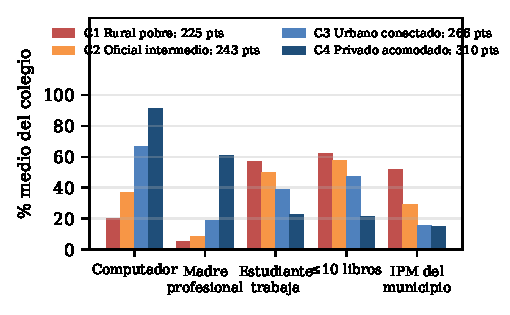
\includegraphics[width=\textwidth]{colegios}
    \end{column}
  \end{columns}
\end{frame}

\begin{frame}{K-means a nivel estudiante: ilustrativo, no robusto}
  \begin{columns}
    \begin{column}{0.5\textwidth}
      \begin{itemize}
        \item Con $k = 3$ (semilla 42): privado acomodado, 20,8\,\%, 291,3 puntos;
        oficial mayoría mujeres, 58,9\,\%, 245,2 puntos; oficial mayoría hombres,
        20,3\,\%, 258,7 puntos.
        \item \textbf{Pero no son estables:} el ARI entre la semilla 42 y las
        semillas 1 y 7 es 0,17 y 0,02.
        \item Los perfiles describen una sola corrida. La conclusión útil sale
        del nivel colegio.
      \end{itemize}
    \end{column}
    \begin{column}{0.5\textwidth}
      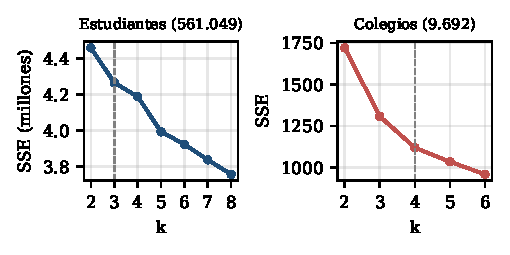
\includegraphics[width=\textwidth]{codo}
    \end{column}
  \end{columns}
\end{frame}

\begin{frame}{Técnica 2: clasificación con J48}
  \begin{columns}
    \begin{column}{0.5\textwidth}
      \begin{itemize}
        \item Predice Alto/Bajo sobre la mediana (254). Validación cruzada
        de 10 particiones, 48 atributos.
        \item \textbf{Exactitud 70,71\,\%}, kappa 0,414, AUC 0,769
        (ZeroR: 50,15\,\%).
        \item Sin cruces: 70,45\,\%; con solo 18 atributos de 2022: 68,74\,\%.
        \item Raíz del árbol: el NSE del colegio. NSE4 $\Rightarrow$ Alto
        (92\,\% de acierto); NSE1 $\Rightarrow$ Bajo (76\,\%).
        \item El estrato del hogar apenas aparece en el puesto 23.
      \end{itemize}
    \end{column}
    \begin{column}{0.5\textwidth}
      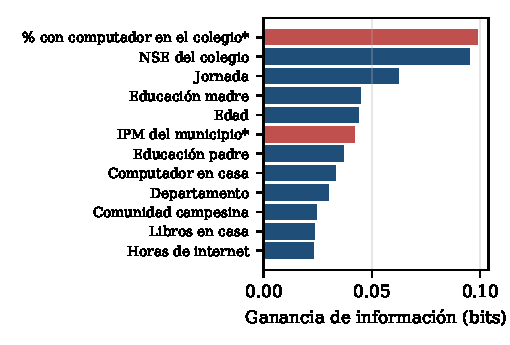
\includegraphics[width=\textwidth]{infogain}
    \end{column}
  \end{columns}
\end{frame}

\begin{frame}{Hallazgo central: el colegio pesa más que el hogar}
  \begin{columns}
    \begin{column}{0.48\textwidth}
      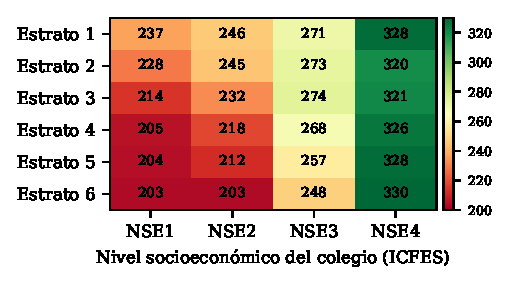
\includegraphics[width=\textwidth]{estrato_nse}
    \end{column}
    \begin{column}{0.52\textwidth}
      \begin{itemize}
        \item Estrato 1: \textbf{237 puntos} en colegio NSE1 y
        \textbf{328} en colegio NSE4: \textbf{+91 puntos}.
        \item Brechas: computador en casa +30,2; privado/oficial +27,7;
        urbano/rural +23,9; género +8,9 (era 7,3 en 2022).
        \item Trabajar $>$30 h/semana: $-$34 puntos. Más de 100 libros: +42,2.
        Leer 30--60 min: +15,3.
        \item IPM $<$20: 268,1 puntos; IPM $>$50: 223,8.
      \end{itemize}
    \end{column}
  \end{columns}
\end{frame}

\begin{frame}{Técnica 3: bandit contextual, el tutor virtual}
  \begin{columns}
    \begin{column}{0.52\textwidth}
      \begin{itemize}
        \item LinUCB elige qué área reforzar para cada estudiante.
        La recompensa es el rezago en esa área: identifica el área más débil,
        no demuestra que reforzarla mejore el puntaje.
        \item Arrepentimiento vs.\ azar: \textbf{$-$14,6\,\%}
        (319.585 $\rightarrow$ 272.944). Área óptima: \textbf{26,1\,\%}
        frente a 20,0\,\% del azar.
        \item Política: inglés en oficiales (44\,\%), rurales (58\,\%) e
        IPM $>$50 (55\,\%); matemáticas en privados (34\,\%).
      \end{itemize}
    \end{column}
    \begin{column}{0.48\textwidth}
      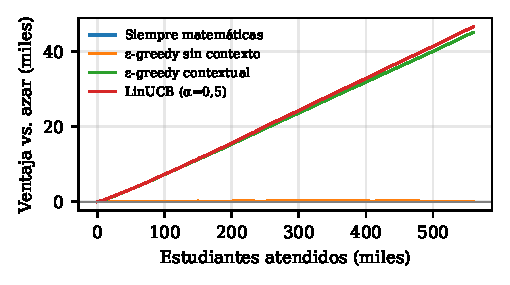
\includegraphics[width=\textwidth]{bandit}
    \end{column}
  \end{columns}
\end{frame}

\begin{frame}{Comparación con 2022 y entre técnicas}
  \begin{columns}
    \begin{column}{0.55\textwidth}
      \small
      \begin{tabular}{lrr}
        \toprule
        & 2022 & 2025 \\
        \midrule
        Estudiantes analizados & 530.815 & 561.049 \\
        Atributos / cruces & 18 / no & 48 / sí \\
        Mediana puntaje global & 247 & 254 \\
        Brecha computador & 31,7 & 30,2 \\
        Brecha privado/oficial & 28,8 & 27,7 \\
        Brecha urbano/rural & 25,8 & 23,9 \\
        J48, mejor & 69,2\,\% & 70,7\,\% \\
        Mejor bandit vs.\ azar & $-$12,3\,\% & $-$14,6\,\% \\
        \bottomrule
      \end{tabular}
    \end{column}
    \begin{column}{0.45\textwidth}
      Las tres técnicas coinciden:
      \begin{enumerate}
        \item El contexto del colegio pesa más que el del hogar.
        \item La pobreza del territorio se suma.
        \item El perfil no predice bien a cada persona
        (70,7\,\%; 26,1\,\% de acierto del bandit).
      \end{enumerate}
    \end{column}
  \end{columns}
\end{frame}

\begin{frame}{Conclusiones}
  \begin{itemize}
    \item El desempeño se asocia sobre todo con el contexto del colegio
    (NSE y compañeros con computador), seguido de la jornada, la educación
    de la madre, la edad y la pobreza del municipio.
    \item Trabajar durante el bachillerato, tener pocos libros y no leer por
    gusto se asocian con puntajes más bajos.
    \item Las brechas casi no cambiaron entre 2022 y 2025.
    \item Todo son \textbf{asociaciones, no causas}.
    \item Trabajo futuro: seguir esta cohorte hasta Saber Pro cuando esté
    disponible, y comparar con Random Forest.
  \end{itemize}
  \vspace{0.4cm}
  \centering
  Código y resultados: \url{https://github.com/its-camilo/saber11-aprendizaje-maquinal}

  \vspace{0.2cm}
  \textbf{¡Muchas gracias!}
\end{frame}

\end{document}
